\documentclass{article}
\usepackage[utf8]{inputenc}
\usepackage{float}
\usepackage{authblk}

\title{Structuring and Analysing Voting within the European Parliament}
\author[1]{ Ross Chadwick }
\affil[1]{(Department of Computer Science, Vrije Universiteit Amsterdam)}
\date{June 2018 (Draft)}

\usepackage[firstpage]{draftwatermark}
\usepackage[numbers]{natbib}
\usepackage{graphicx}
\usepackage{subcaption}
\usepackage{url}
\usepackage{hyperref}
\usepackage{notoccite}
\usepackage{placeins}

\begin{document}
\maketitle

\section{Introduction}
Beginning in 2001, a European regulation was passed providing public access rights to all documents produced by the European Parliament, Council and Commission 
\cite{EURegulation2001}.
The information published by these European institutions provides rich resources for many scientific disciplines. Ranging from insights into large-scale politics 
\cite{Hoyland2014PredictingPA, Greene2015UnveilingTP, Hix2009VotingPA}, human-behaviour analysis \cite{Meserve2007PoliticalAA}, social-network analysis 
\cite{Cherepnalkoski2016RetweetNO, Cherepnalkoski2016CohesionAC, Cherepnalkoski2015ARN, NetworksAttila} and natural language processing (NLP) \cite{Koehn2005EuroparlAP, 
Hajlaoui2014DCEPC}.
\newline
Although such information is publicly available, it is mostly provided in an unstructured manner and in a variety of formats. A large amount of research time could be mitigated if 
European Union data could transition to 5 star linked open data.
\newline
\newline
Within this research project, I will focus on the topic of voting within the European Parliament. Specifically, by modelling behaviour at the lowest level of abstraction; individual 
Members of Parliament's (MEP's) votes. \textbf{Modelling vote relations on an individual basis will potentially open opportunities to perform in-depth analysis into how MEPs form 
stances on vote topics.} I therefore propose to model the legislative process of a dossier passing through the European Parliament, in conjunction with all related activities, 
documents and votes as Linked Open Data (LOD).
\textbf{I then propose to utilise this LOD to provide statistical insights, as well as classifying the stances (opinions) MEPs hold towards topics they vote on, potentially leading 
to a probabilistic vote prediction model.}

\section{Research Goals}
This research proposal therefore has two main goals. Firstly to enrich current understanding of the European Parliament legislative process, by providing machine-readable data with 
links to many external resources. This goal will be assessed by providing in-depth statistical analysis of the types of data available, compared to existing data-sets.
\newline
Secondly, the research aims to utilise the produced linked-data to provide a corpus for use in sentiment analysis. This goal will be assessed by testing the accuracy of stance 
(opinion) detection that an MEP holds on certain topics. A second success metric of this goal could then be to use a probabilistic method of predicting the outcome of an MEP's vote 
on a particular topic, based on their stances towards it. This prediction would then be compared to the actual outcome of their vote once it has been published.

\section{Background}
\subsection{Voting and Related Data}
There exists many initiatives focused on utilising and improving European Union data. Very few however touch on the subject of voting outcomes. VoteWatch \cite{votewatch} and 
Parltrack \cite{parltrack} are two notable initiatives aiming to improve the accessibility of European Parliament voting data. While both do mostly reach their goals, they fail to 
cater towards the academic community by not providing well structured data, or by imposing strict licensing.
\newline
LOD related to the European Union is still largely unavailable. There exists one official initiative by the European Council \cite{EUCouncilLOD} which does in-fact provide voting 
data from the council, as well as metadata of requested council documents. Another LOD initiative, with the goal of providing structured data on European Parliament plenary debates 
has been published by Aggelen, Hollink et al. \cite{LinkedPolitics}. In the case of the latter initiative, is has been shown that such information has a demand, with 7500 unique 
queries executed within the first seven months of the data publication \cite{Aggelen2017TheDO}.
\newline
Many relevant resources related to the European Union do already have a presence on the Semantic Web. For example, DBPedia contains many triples on European Parliament political 
groups and MEPs. Typically this information ranges from textual descriptions of the entity and their affiliations with other entities, with very little domain specific information. 
MEP resources do sometimes contain useful properties such as relations within national political groups as well as European Parliament political groups \cite{DBPediaExample}.

\subsection{NLP, Sentiment Analysis and Stance Detection} \label{backgroundNLP}

Belford et al. \cite{Belford2016TweetingEA} performed unsupervised topic modelling on the tweets of MEPs. Their model comprised of ensemble learning over multiple layers of 
Non-negative Matrix Factorisation (NMF). Such a technique has proven to be a successful approach to annotating topics of texts in an unsupervised manner. The resulting annotations 
were then used to quantify the attention of MEPs on particular topics over time.
\newline
\newline
Zhang et al. \cite{Zhang2016GatedNN} propose a deep learning model for sentence-level sentiment analysis, allowing for targeted sentimental analysis of text. The concept of targeted 
sentiment analysis allows for the classification of polarity towards separate targets within a text, instead of the text as a whole. Their model was tested on tweets with an explicit 
target entity and achieved accuracy of 71.96 percent.
\newline
\newline
Mohammad et al. \cite{Mohammad2017StanceAS} have made some interesting insights into document-level sentiment analysis and how a person's stance towards an entity can comprise of 
both positive and negative sentiment, pointing out a clear separation between the sentiment polarity and a person's stance. The authors propose a supervised support vector machine 
(SVM) model, which achieves up to 70 percent accuracy on their test data. Zarrella et al. \cite{Zarrella2016MITREAS} propose an approach relying on recurrent neural networks (RNN), 
which they tested against the same data-set. The RNN approach resulted in a slightly lower accuracy of 67 percent. It achieved such a score with only 2,814 training tweets, which is 
a very small sample size for training such a model. Rakholia et al. \cite{Rakholia2017IsIT} further this work and produce a comparison of deep learning models for the task of stance 
detection on the same data-set.

\subsection{Vote Prediction Models}
\textit{TBD if this will remain in scope of this research.}

\section{Methodology}
\subsection{European Parliament Linked Open Data} \label{methodLOD}
\begin{enumerate}
    \item All relevant information on procedures in Parliament will be scraped and converted into linked data, with an accompanying ontology to assist in the inference of relations. 
Parltrack provides in-depth data-sets \cite{parltrackSchema} (Open Database License) scraped from the official Parliament website, reducing the need to build custom scrapers.
    \item The ontology will be modelled with immutability in mind, to mitigate the likelihood of triples requiring updates.
    \item A system will be built that will allow for regular automatic extension of the data-set.
    \item Resources will be linked to their external counterparts where available (DBPedia, LinkedEP, GeoNames, European Council, JRC-Names):
    \begin{enumerate}
        \item DBPedia - MEPs, political groups and locations will be linked to their existing DBPedia Resource (DBR).
        \item LinkedEP - MEPs will be linked to their resource. LinkedEP AgendaItem resources will be linked to their corresponding procedural activity.
        \item GeoNames - All locational resources, will be linked to their GeoNames resource for a wider range of geographical information on dossiers and people.
        \item European Council - When the European Council has had voting involvement within a procedure, the relevant resources will be linked to.
        \item JRC-Names \cite{Ehrmann2017JRCNamesME} - MEP resources will be linked to their JRC-Names resource where available, to provide access to variations of their names. This 
should greatly improve the ability of querying over MEPs in a multilingual fashion.
    \end{enumerate}
    \item Textual resources will be annotated with mentioned resources using tools such as DBPedia Spotlight \cite{isem2013daiber}, GATE \cite{} and possibly a custom topic modelling 
solution.
\end{enumerate}

\subsection{Stance Detection of MEPs} \label{methodStance}
As discussed in section \ref{backgroundNLP}, stance detection requires sentence-level sentiment analysis, to determine the target of a sentence's polarity. It is still to be 
determined whether stance detection will be applied to texts as a whole, where the target is the document in question or if each target in said document shall have a stance 
associated with it.

\begin{enumerate}
    \item Textual data, both from the produced data-set and external resources will be gathered for each vote and opinion an MEP has made. Some examples include:
    \begin{enumerate}
        \item Written explanations for an MEP's vote \cite{exampleExplanations} - A written explanation is often given by an MEP and translated from their first language to all other 
European languages. These explanations can be classified according to the type of vote (For, Against, Abstain) that accompanies them. Written explanations should therefore form a 
large basis of any domain specific training data needed for supervised stance detection.
        \item Debate transcripts \cite{exampleDebate} - Before any voting round has commenced, at least one debate will have taken place, with many MEPs verbally giving their opinion 
on the subject at hand. This is once again translated from their first language to every other European language. These debate texts will form the basis of the test data being 
classified by the stance detection model.
        \item Twitter messages - A majority of current MEPs utilise Twitter to share their personal opinions outside of Parliament. It will be explored if these tweets can prove 
useful during sentiment analysis.
    \end{enumerate}
    \item Link prediction techniques could alternatively be utilised in order to predict an MEP's stance on a particular topic, avoiding the need for sentiment analysis. (More 
research is required)
\end{enumerate}

\subsection{Prediction of Future Votes} \label{methodPrediction}
\textit{TBD if this will remain in scope of this research.}
\newline
\newline
A probabilistic model would be designed to take into account the previously classified stances an MEP holds towards certain topics. Secondly, any new opinions on the topic that will 
have a vote, will be classified. At this stage, we may already see notable shifts in stance, by comparing previous stances to the current stance on each topic. Past and current 
stances towards the topics to be voted on can then be weighted appropriately to create a probability distribution across the three possible voting outcomes (For, Against, Abstain). 

\section{Potential Problems}
\textit{This section is a work in progress and shall be expanded on as my research continues.}
\newline
\newline
The basis of my second goal relies on the assumption that an MEP's stance (opinion) on a topic directly corresponds to the type of vote that they will make. However researchers such 
as Hix et al. \cite{Hix2009VotingPA} discuss the fact that an MEP's vote may not always reflect their exact opinion on the matter, but is in-fact influenced by their affiliated 
political group. This question will need more investigation to determine whether or not it could have negative influence on my results.


\section{Preliminary Work}
Work is already well underway modelling the ontology and producing triples of some aspects that will be considered. A prototype implementation of the data mining tool which produces 
said triples and updates a SPARQL endpoint with them is fully functional and outputs around 20 million triples (including basic OWL2-RL inferences). The tool currently relies on the 
Parltrack data-sets and does not do any scraping itself. It will be explored if this is a reasonable way to continue, or if the Parltrack scraping tools will be forked and customised 
to allow complete control over the scraping process.
\newline
Figure \ref{fig:mepGraph} demonstrates an example visualisation of some of the triples currently available for an MEP resource. In this example, the target resource is in fact a 
DBPedia resource for Terry Reintke, which has inherited properties through an $owl:sameAs$ relation to the internal MEP resource. The figures following show the current properties 
that the most notable resources in the graph contain. 
\newline
Firstly we can see that this MEP has some basic properties associated (\ref{fig:propertiesMEP}), such as birth date, gender and name. The MEP then has a membership 
(\ref{fig:propertiesMembership}), showing that they represent Germany within the Verts/ALE political group as of 01-07-2014. The absence of an end date indicates that this membership 
is still active. Next we see a reaction (\ref{fig:propertiesReaction}) that this MEP has made towards a voting round, in which they voted "For" as indicated by the reaction having 
type $epv:VoteFor$. We can then see some basic information on the voting round in question (\ref{fig:propertiesVote}). Looking further we can follow the relations of the vote, all 
the way to the dossier (procedure) that it applies to (\ref{fig:propertiesDocument}, \ref{fig:propertiesActivity}, \ref{fig:propertiesDossier}).


\begin{figure}
  \centering
  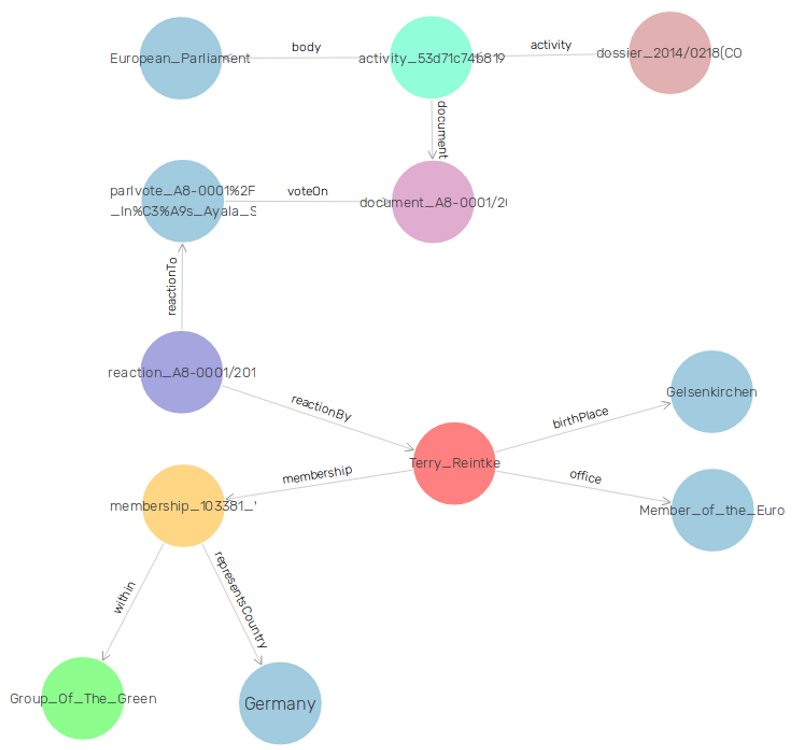
\includegraphics[width=1\linewidth]{images/graph.png}
  \caption{Example MEP (Terry Reintke) and a subset of their relations}
  \label{fig:mepGraph}
\end{figure}

\begin{figure}
\begin{subfigure}{.5\textwidth}
  \centering
  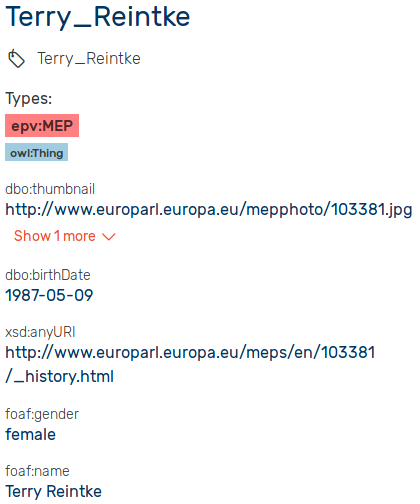
\includegraphics[width=.8\linewidth]{images/mep.png}
  \caption{MEP Properties}
  \label{fig:propertiesMEP}
\end{subfigure}%
\begin{subfigure}{.5\textwidth}
  \centering
  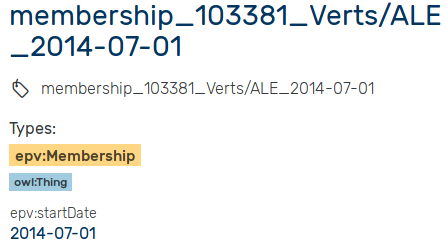
\includegraphics[width=.8\linewidth]{images/membership.png}
  \caption{MEP Membership Properties}
  \label{fig:propertiesMembership}
\end{subfigure}
\label{fig:fig}
\end{figure}

\begin{figure}
\begin{subfigure}{.5\textwidth}
  \centering
  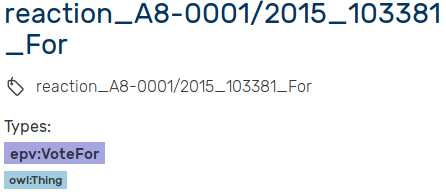
\includegraphics[width=.8\linewidth]{images/reaction.png}
  \caption{MEP's vote "For"}
  \label{fig:propertiesReaction}
\end{subfigure}%
\begin{subfigure}{.5\textwidth}
  \centering
  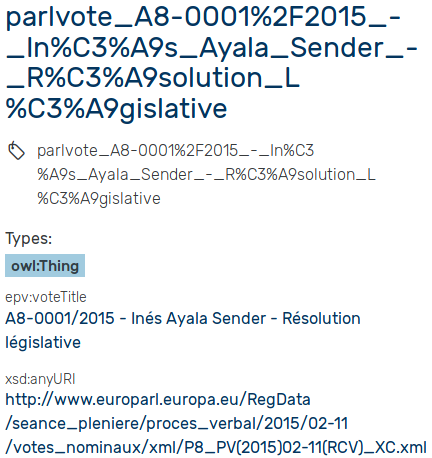
\includegraphics[width=.8\linewidth]{images/vote.png}
  \caption{The vote in parliament which the MEP reacted to}
  \label{fig:propertiesVote}
\end{subfigure}
\label{fig:fig}
\end{figure}

\begin{figure}
\begin{subfigure}{.33\textwidth}
  \centering
  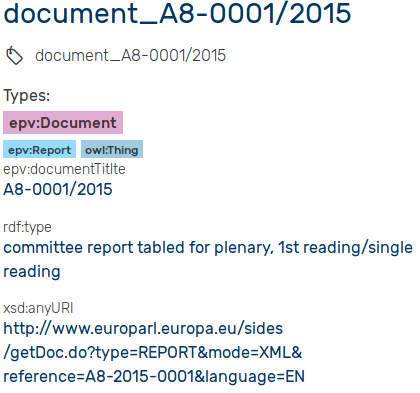
\includegraphics[width=\linewidth]{images/document.png}
  \caption{The report which was the basis of the vote}
  \label{fig:propertiesDocument}
\end{subfigure}%
\begin{subfigure}{.33\textwidth}
  \centering
  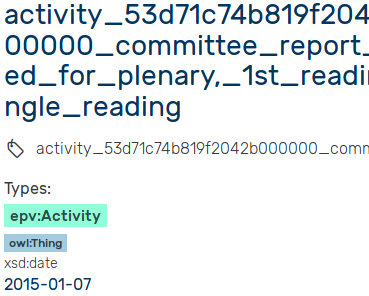
\includegraphics[width=\linewidth]{images/activity.png}
  \caption{The parliamentary activity of which the document belongs to}
  \label{fig:propertiesActivity}
\end{subfigure}
\begin{subfigure}{.33\textwidth}
  \centering
  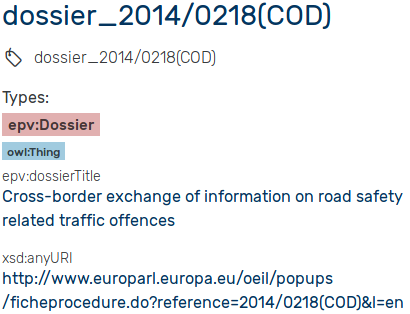
\includegraphics[width=\linewidth]{images/dossier.png}
  \caption{The dossier which the activity was in regards to}
  \label{fig:propertiesDossier}
\end{subfigure}
\label{fig:propertiesDocDossier}
\end{figure}

\FloatBarrier
\bibliographystyle{unsrtnat}
\bibliography{references}
\end{document}
